\documentclass[sigconf]{acmart}

% ── ACM Metadata ──────────────────────────────────────────
\acmConference[]{}{}{}
\acmYear{2025}
\acmISBN{978-x-xxxx-xxxx-x/25/MM}
\acmDOI{10.1145/xxxxxxx.xxxxxxx}

\copyrightyear{2025}
\setcopyright{acmlicensed}

% Remove "Authors' Contact Information" and "Permission to make..." footnotes
\renewcommand\footnotetextcopyrightpermission[1]{}
\settopmatter{printacmref=false, printfolios=false}

% ── CCS Concepts ──────────────────────────────────────────
\begin{CCSXML}
<ccs2012>
  <concept>
    <concept_id>10010147.10010257.10010293.10010294</concept_id>
    <concept_desc>Computing methodologies~Text classification</concept_desc>
    <concept_significance>500</concept_significance>
  </concept>
  <concept>
    <concept_id>10010147.10010257.10010293</concept_id>
    <concept_desc>Computing methodologies~Classification and regression trees</concept_desc>
    <concept_significance>300</concept_significance>
  </concept>
</ccs2012>
\end{CCSXML}

\ccsdesc[500]{Computing methodologies~Text classification}
\ccsdesc[300]{Computing methodologies~Classification and regression trees}

\keywords{Noise Robustness, Natural Language Processing, character-level noise,
Logistic Regression, Naive Bayes, Support Vector Machine, Ensemble Methods,
TF-IDF, out-of-vocabulary tokens, SST-2, Sentiment Analysis}

% ══════════════════════════════════════════════════════════
\begin{document}

% ── Title & Authors ───────────────────────────────────────
\title{A Comparative Analysis of Classifier Robustness to Character-Level Noise in Sentiment Analysis}

\author{Karthika Veeravaneni}
\affiliation{%
  \institution{Your Institution}
  \city{City}
  \country{Country}
}
\email{your.email@institution.edu}

\author{Venkata Naga Sai Yaswanth Deevi}
\affiliation{%
  \institution{Your Institution}
  \city{City}
  \country{Country}
}
\email{your.email@institution.edu}

% ── Abstract ──────────────────────────────────────────────
\begin{abstract}
Sentiment analysis models are typically trained and evaluated on clean,
well-formed text. However, real-world user input frequently contains
character-level noise from typographical errors, hasty typing, and mobile
keyboards. This paper presents a systematic, quantitative comparison of four
classifiers: Logistic Regression (LR), Multinomial Naive Bayes (MNB), Linear
SVM, and a Hard-Voting Ensemble, on the Stanford Sentiment Treebank (SST-2)
under three types of character-level noise (character swap, deletion, and
keyboard-neighbour substitution) at five intensities ranging from 5\% to 25\%,
evaluated across five random seeds. All models degrade monotonically with
increasing noise; character deletion causes the largest drops, reaching
$\Delta$Acc $= 0.141$ for MNB at 25\% intensity. The hard-voting ensemble ranks
first on raw $\Delta$Acc in two of three noise conditions, but its margins over
Logistic Regression are within one standard deviation throughout, and under
character deletion, LR is actually more robust. The clearest finding is that
MNB is the most fragile compared to the other classifiers. LR, SVM, and the
Ensemble perform similarly under noise. These results highlight that
clean-data accuracy does not guarantee robustness.
\end{abstract}

\maketitle

% ──────────────────────────────────────────────────────────
\section{Introduction}

Natural Language Processing models for tasks such as sentiment analysis are
trained on clean and curated datasets. In deployment, however, models are given
text that is hastily typed on mobile phones, corrupted during data collection,
or generated by non-native speakers, resulting in different types of
character-level errors. Therefore, understanding how such noise affects the
performance of the classifier is imperative.

Although there is a lot of research on comparing classifier accuracy on clean
datasets, there is relatively little research on comparing the robustness of
classifiers. Few studies that address noise robustness tend to focus on a
single noise type or a single classifier, making it difficult to draw general
conclusions. This research gap motivates the present work.

A similar issue appears in related preprocessing tasks. Tumula \&
Nerusu~\cite{tumula2024} show that in healthcare data imputation, the
preprocessing method you choose can significantly change how models behave
later, even if the accuracy looks the same. They found that simpler methods
like KNN can sometimes be more robust than advanced deep learning methods such
as VAE and GAN when the focus is on robustness rather than just accuracy. This
supports our hypothesis that combining classical classifiers in an ensemble may
perform better than relying on a single strong model, especially under noisy
conditions.

\subsection*{Research Questions}

\textbf{RQ1:} How do the type and intensity of character-level noise affect the
accuracy and F1-score of Logistic Regression, Multinomial Naive Bayes, and
Linear SVM on binary sentiment analysis?

\textbf{RQ2:} Does a hard-voting ensemble of the three classifiers provide
better robustness than the strongest individual model, and are any performance
gains statistically significant across different random seeds?


% ──────────────────────────────────────────────────────────
\section{Related Work}

\subsection{Noise Robustness in NLP}
Wang \& Manning~\cite{wang2012} showed that TF-IDF with bigrams and simple
linear classifiers can do very well on clean sentiment classification and topic
classification tasks. However, they did not take noisy inputs into
consideration. Walker et al.~\cite{walker2010} looked at how OCR errors, which
are a type of character-level mistake, can hurt topic models and found that
even a small number of errors can have a big effect. Their work is one reason
why this study focuses on character-level noise.

\subsection{Classifier Comparison and Fusion}
Solovyeva et al.~\cite{solovyeva2022} compare several machine learning methods
for text classification and show that no single classifier performs best in all
situations. Moreno-Seco et al.~\cite{moreno2006} provide both theoretical and
experimental evidence that combining classifiers using hard voting can reduce
variance and improve robustness without extra training. Tujantri et
al.~\cite{tujantri2025} extend this line of work to hyperparameter-tuned SVM
and Naive Bayes, finding that performance gaps between classifiers narrow under
distribution shift.

\subsection{Accuracy vs.\ Robustness Trade-offs}
A common finding in preprocessing and model evaluation studies is that
optimising for accuracy on a clean test set does not ensure robustness under
distribution shift. Tumula \& Nerusu~\cite{tumula2024} show this in data
imputation: GANs and VAEs have lower imputation error than KNN but cause much
more demographic bias.


% ──────────────────────────────────────────────────────────
\section{Methodology}

\subsection{Dataset and Feature Extraction}
This experiment uses the \textbf{Stanford Sentiment Treebank v2 (SST-2)}, a
standard binary sentiment benchmark containing 67,000 training sentences and
1,821 test sentences drawn from movie reviews. All models use the same TF-IDF
vectorisation setup: unigrams and bigrams, sublinear term-frequency scaling,
and a maximum document frequency of 0.95. The vectorizer is fitted only on the
clean training data and kept fixed for all evaluations, ensuring that no
information from the noisy test data leaks into the features.

\subsection{Noise Generation}
Three character-level noise functions are applied independently to each
character in the test set with probability
$p \in \{0.05, 0.10, 0.15, 0.20, 0.25\}$:

\begin{itemize}
  \item \textbf{Character swap:} two adjacent characters within a word are
    transposed (e.g., \textit{film} $\to$ \textit{iflm}).
  \item \textbf{Character deletion:} a randomly selected alphabetic character
    is removed (e.g., \textit{film} $\to$ \textit{fim}).
  \item \textbf{Keyboard-neighbour substitution:} a character is replaced by a
    physically adjacent key on a QWERTY layout (e.g., \textit{film} $\to$
    \textit{fikm}).
\end{itemize}

These three types cover the most common real-world typing errors: swapped
letters, missing keys, and hitting the wrong nearby key.

\subsection{Classifiers}
Four models are evaluated:

\begin{itemize}
  \item \textbf{Logistic Regression (LR):} $\ell_2$-regularised, LBFGS
    solver, $C = 1.0$.
  \item \textbf{Multinomial Naive Bayes (MNB):} Laplace smoothing,
    $\alpha = 0.1$.
  \item \textbf{Linear SVM:} $\ell_2$ hinge loss, $C = 1.0$.
  \item \textbf{Hard-Voting Ensemble:} majority vote of LR, MNB, and SVM
    predictions.
\end{itemize}

All models are trained once per seed on clean training data and evaluated
across all noisy test variants without retraining. This way, we measure how
noise affects the model's predictions, not how the model adapts. We use five
random seeds (42, 7, 123, 2024, 99) to capture variation in the results.

\subsection{Evaluation Metrics}
Primary evaluation uses accuracy and macro-averaged F1-score. The core
robustness metric is $\Delta$Acc: the absolute drop in accuracy from the 0\%
noise baseline to a given noise condition. Stability across seeds is reported
as standard deviation (SD). Following the principle that accuracy alone is
insufficient for evaluating method quality~\cite{tumula2024}, we consider
$\Delta$Acc and degradation rate as the primary robustness indicators. Paired
$t$-tests ($\alpha = .05$) across 15 non-zero noise conditions check if the
differences between models are statistically significant.


% ──────────────────────────────────────────────────────────
\section{Results}

\subsection{Degradation Curves}
Figure~\ref{fig:mean_deg} shows all four classifiers on the same axis for each
noise type, with shaded bands representing $\pm$1~SD. All models degrade
monotonically: no model improves at higher noise levels. The severity of the
three noise types is the same for all classifiers: character deletion causes
the largest drop, keyboard-neighbour substitution is next, and character swaps
have the smallest effect. This ranking is supported by the $\Delta$Acc values
at 25\% noise across all models (see Table~\ref{tab:robustness}): for every
classifier, deletion $>$ keyboard $>$ swap. Under character deletion, MNB
drops much faster than the other three classifiers from 10\% noise onward.
With character swaps, all four classifiers stay close, reaching about 0.66
accuracy at 25\% noise. Variation between random seeds is small (SD $<$
0.022), showing these trends are stable and not due to a specific data split.

\begin{figure}
  \centering
  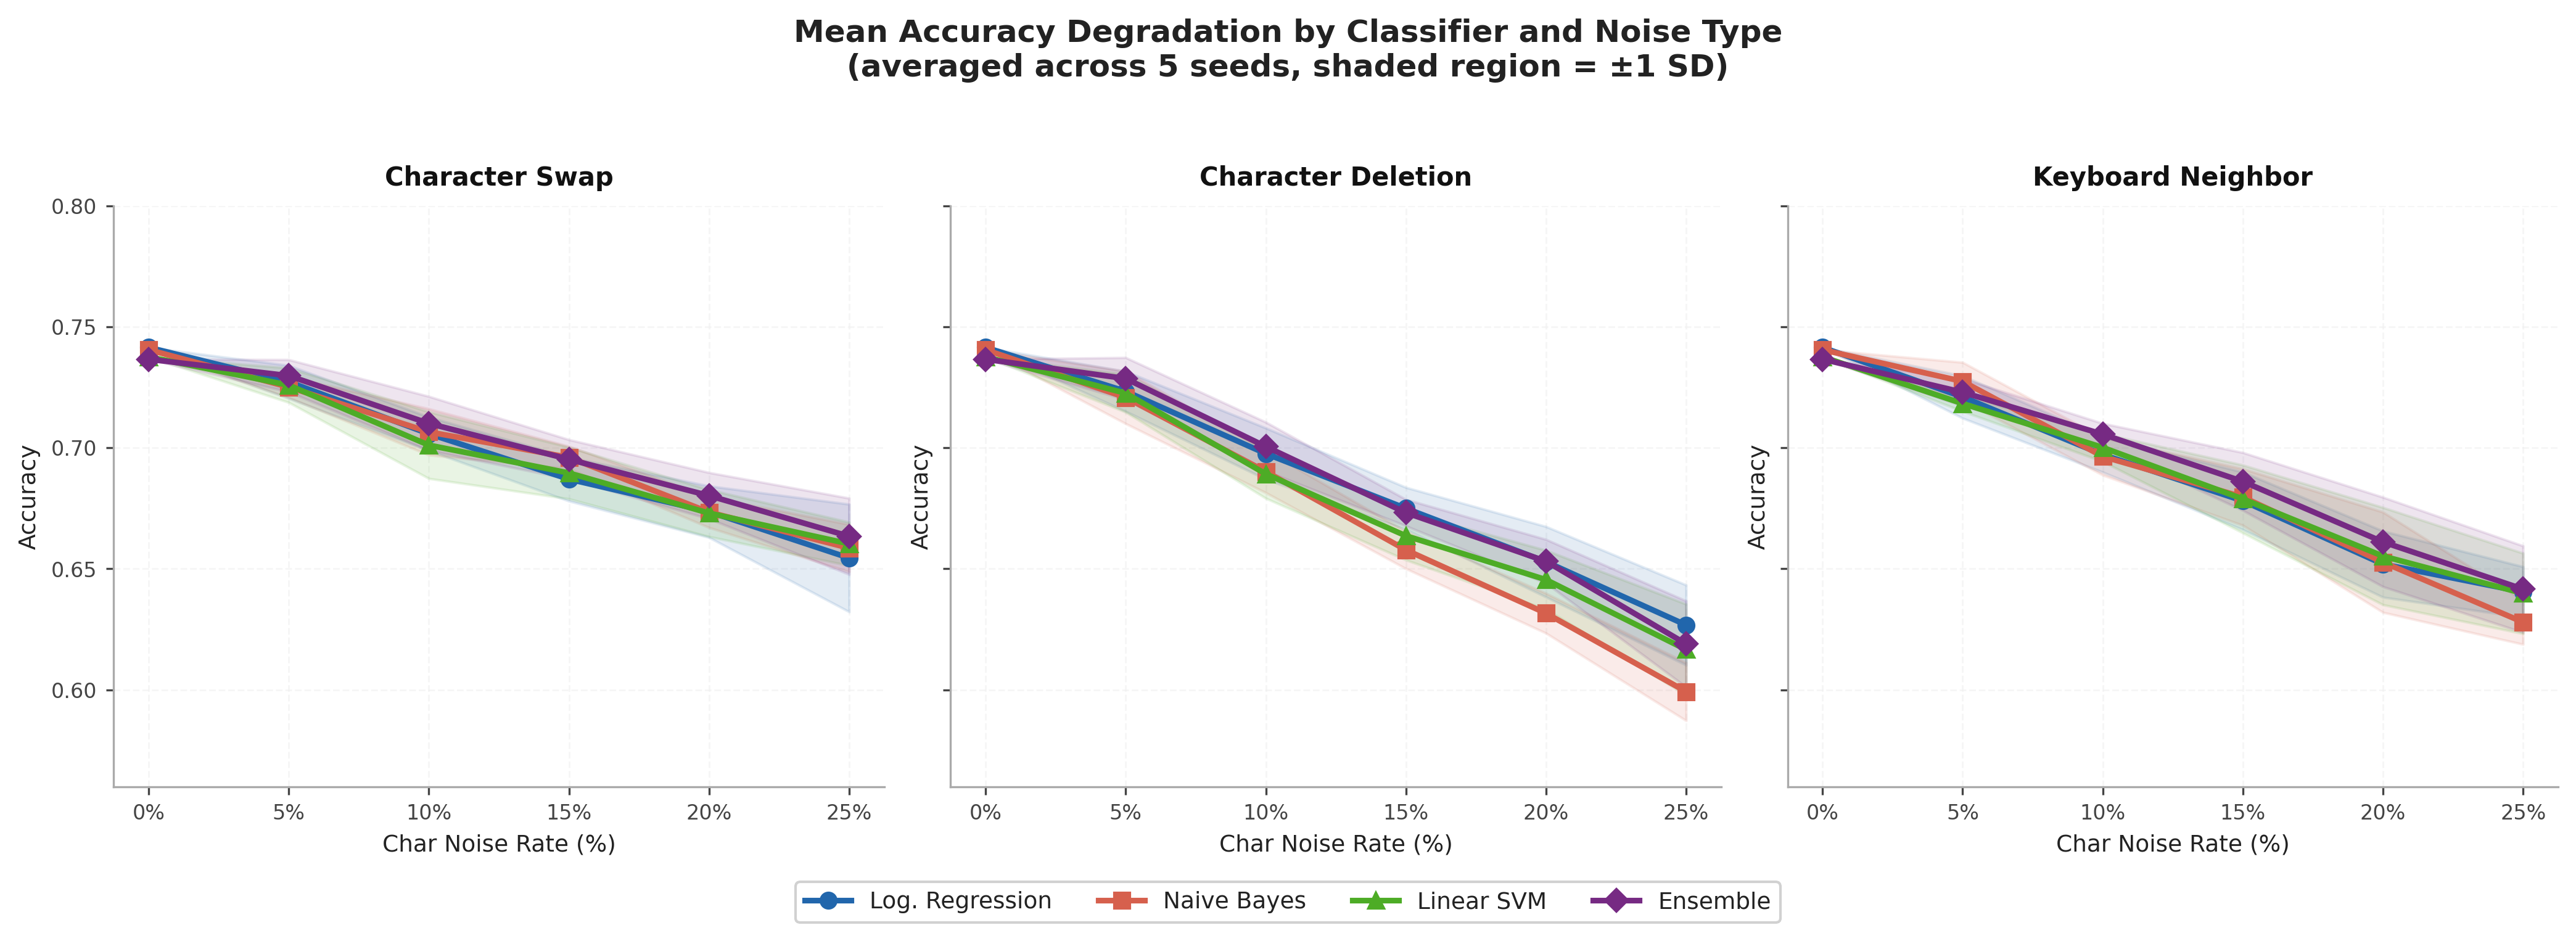
\includegraphics[width=\linewidth, interpolate=false, resolution=300]{06_mean_degradation.png}
  \caption{Mean accuracy with $\pm$1 SD bands, all classifiers overlaid per
  noise type.}
  \label{fig:mean_deg}
\end{figure}

\subsection{Robustness Summary at 25\% Noise}
Figure~\ref{fig:robustness} and Table~\ref{tab:robustness} show the mean
accuracy drop from 0\% to 25\% noise, with $\pm$1 SD error bars. The ensemble
records the lowest mean $\Delta$Acc under character swap (0.073) and
keyboard-neighbour noise (0.095), but is outperformed by LR under character
deletion (ensemble: 0.118, LR: 0.115). Crucially, the margins between the
ensemble and the next-best model are very small in all three conditions: 0.004
under character swap, 0.003 under keyboard-neighbour noise, and the ensemble
actually trails LR by 0.003 under deletion. Since the standard deviations
across seeds are only 0.009--0.022, these differences are too small to be
statistically significant. The more defensible conclusion is that \textbf{LR
and the ensemble are about equally robust}, while MNB is a clear outlier: its
$\Delta$Acc of 0.141 under deletion is 0.020--0.026 points worse than any
other model, which is larger than the usual variation between seeds.

\begin{figure}
  \centering
  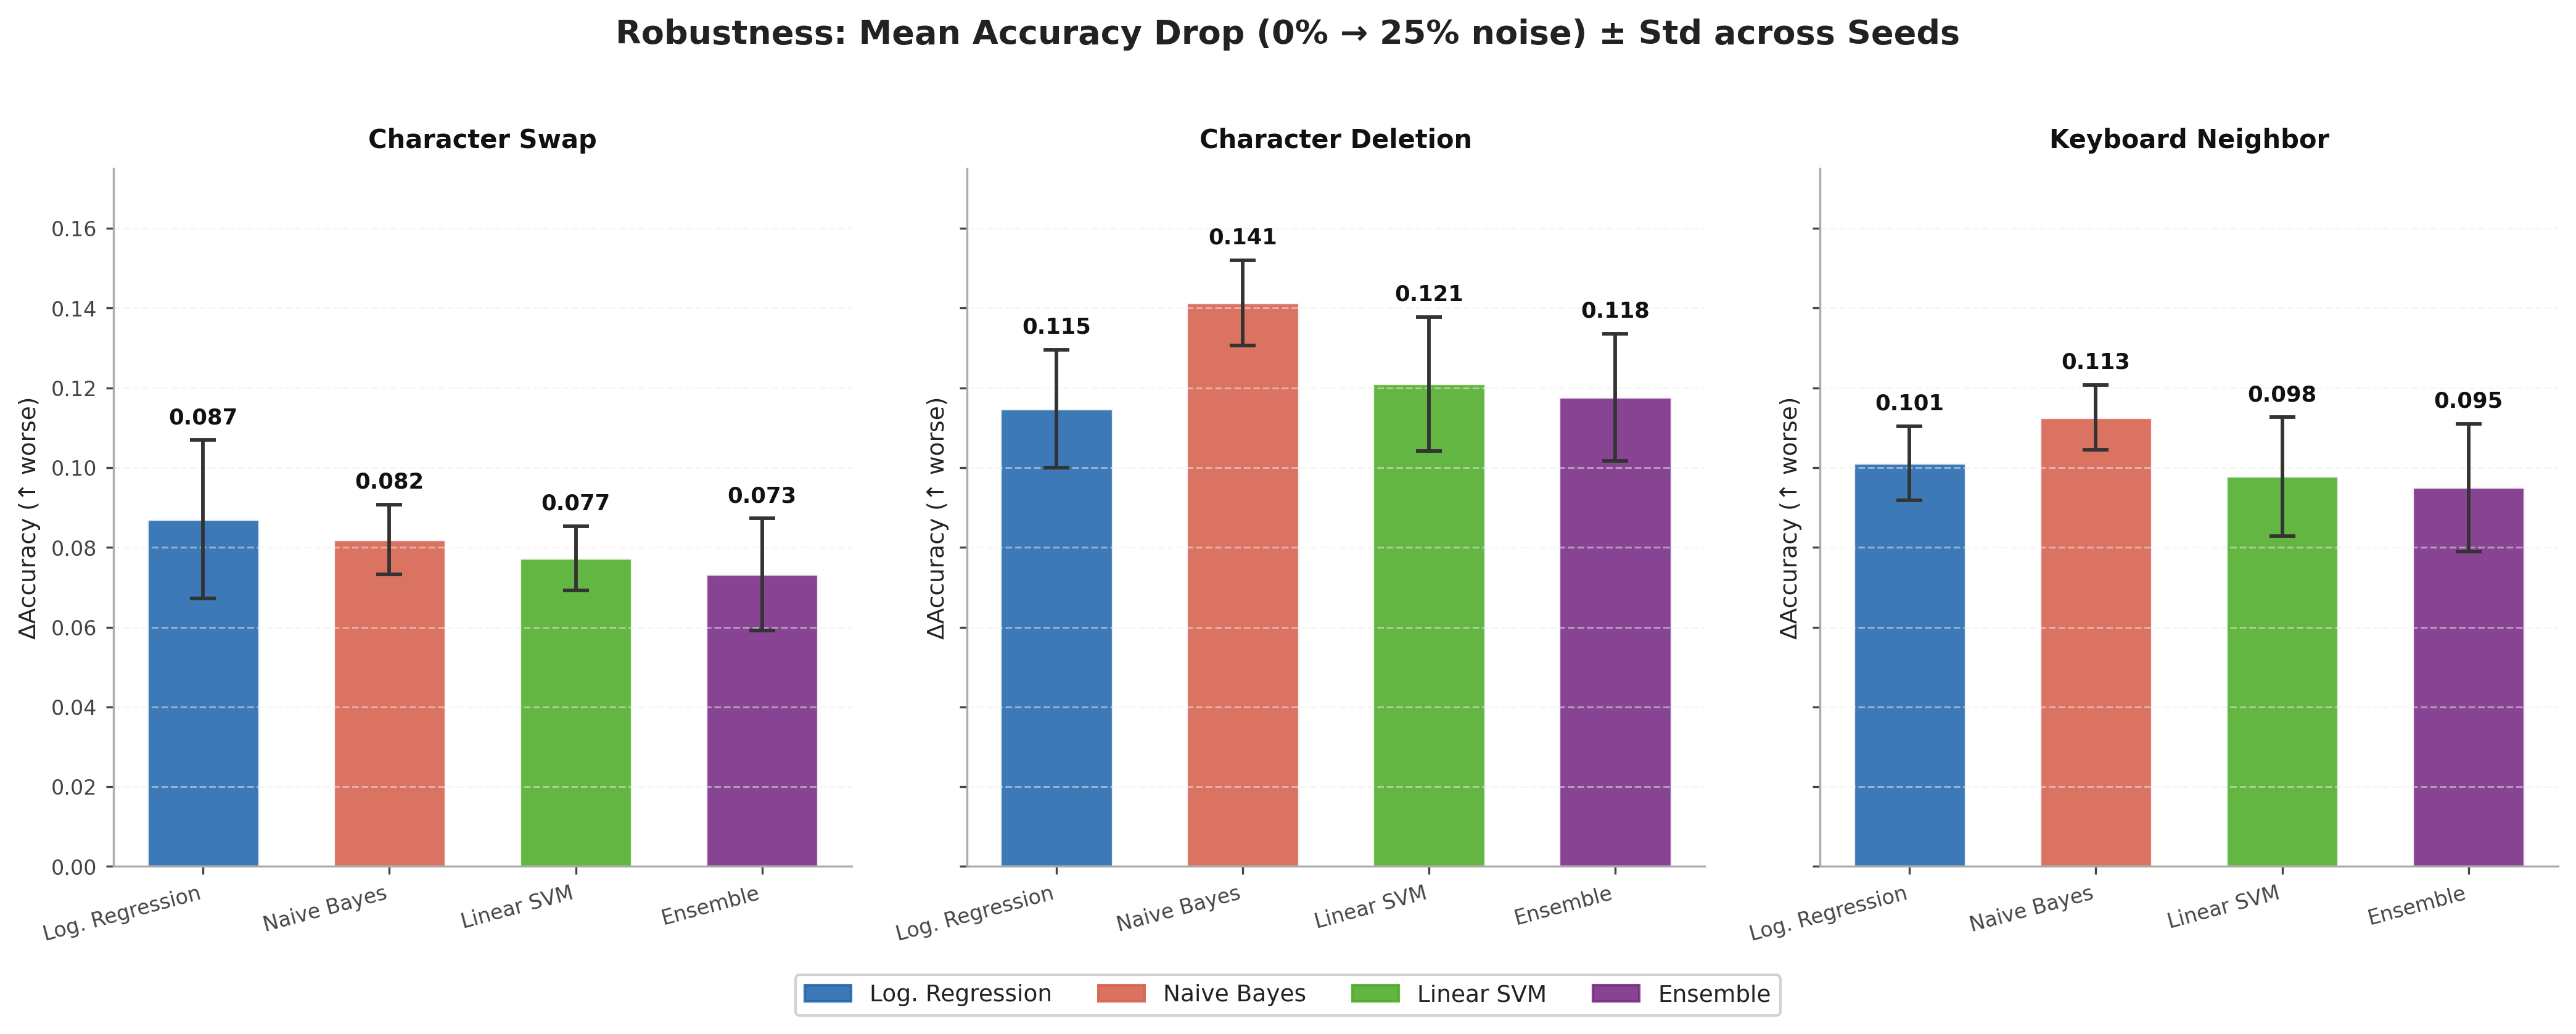
\includegraphics[width=\linewidth, interpolate=false, resolution=300]{05_robustness_drop.png}
  \caption{Mean $\Delta$Acc (0\%$\to$25\%) $\pm$ SD across seeds. Lower bars
  indicate greater robustness.}
  \label{fig:robustness}
\end{figure}

\begin{table}
  \centering
  \caption{Mean $\Delta$Acc at 25\% noise ($\pm$ SD). \textbf{Bold} = most
  robust per row.}
  \label{tab:robustness}
  \small
  \begin{tabular}{lcccc}
    \toprule
    \textbf{Noise} & \textbf{LR} & \textbf{MNB} & \textbf{SVM} & \textbf{Ens.} \\
    \midrule
    Swap     & .087$\pm$.022 & .082$\pm$.010 & .077$\pm$.009 & \textbf{.073$\pm$.016} \\
    Deletion & \textbf{.115$\pm$.017} & .141$\pm$.012 & .121$\pm$.019 & .118$\pm$.018 \\
    Keyboard & .101$\pm$.011 & .113$\pm$.009 & .098$\pm$.017 & \textbf{.095$\pm$.018} \\
    \bottomrule
  \end{tabular}
\end{table}

\subsection{Detailed Results by Noise Type}

Tables~\ref{tab:swap}, \ref{tab:deletion}, and \ref{tab:kbn} report mean
accuracy and F1-score ($\pm$ SD) for character swap, character deletion, and
keyboard-neighbour noise, respectively, across all models and intensity levels.
Bold values mark the best-performing model at each intensity. At the clean
baseline (0\%), LR achieves the highest F1 (0.754), but its advantage
disappears rapidly as noise increases. MNB struggles most with character
deletion: its F1 falls to 0.590 at 25\%, the lowest result in the study and
0.15 below its clean score.

\begin{table}
  \centering
  \caption{Mean Accuracy / F1 ($\pm$ SD): \textbf{Character Swap}.}
  \label{tab:swap}
  \small
  \begin{tabular}{lcccc}
    \toprule
    \textbf{Noise} & \textbf{LR} & \textbf{MNB} & \textbf{SVM} & \textbf{Ens.} \\
    \midrule
    \multicolumn{5}{l}{\textit{Accuracy}} \\
    0\%  & \textbf{.742} & .741 & .738 & .737 \\
    5\%  & .727$\pm$.007 & .725$\pm$.004 & .726$\pm$.007 & \textbf{.730$\pm$.007} \\
    10\% & .706$\pm$.007 & .707$\pm$.010 & .701$\pm$.014 & \textbf{.710$\pm$.011} \\
    15\% & .687$\pm$.009 & .696$\pm$.005 & .690$\pm$.011 & \textbf{.695$\pm$.008} \\
    20\% & .674$\pm$.011 & .673$\pm$.006 & .673$\pm$.010 & \textbf{.680$\pm$.010} \\
    25\% & .654$\pm$.022 & .659$\pm$.010 & .661$\pm$.009 & \textbf{.664$\pm$.016} \\
    \midrule
    \multicolumn{5}{l}{\textit{F1-Score}} \\
    0\%  & \textbf{.754} & .744 & .747 & .746 \\
    5\%  & .740$\pm$.007 & .729$\pm$.004 & .732$\pm$.006 & \textbf{.737$\pm$.007} \\
    10\% & .719$\pm$.006 & .712$\pm$.012 & .708$\pm$.016 & \textbf{.718$\pm$.012} \\
    15\% & .701$\pm$.009 & .700$\pm$.007 & .695$\pm$.012 & \textbf{.704$\pm$.008} \\
    20\% & .688$\pm$.012 & .678$\pm$.006 & .675$\pm$.013 & \textbf{.688$\pm$.011} \\
    25\% & .670$\pm$.022 & .666$\pm$.012 & .660$\pm$.010 & \textbf{.673$\pm$.016} \\
    \bottomrule
  \end{tabular}
\end{table}

\begin{table}
  \centering
  \caption{Mean Accuracy / F1 ($\pm$ SD): \textbf{Character Deletion}.}
  \label{tab:deletion}
  \small
  \begin{tabular}{lcccc}
    \toprule
    \textbf{Noise} & \textbf{LR} & \textbf{MNB} & \textbf{SVM} & \textbf{Ens.} \\
    \midrule
    \multicolumn{5}{l}{\textit{Accuracy}} \\
    0\%  & \textbf{.742} & .741 & .738 & .737 \\
    5\%  & .723$\pm$.008 & .721$\pm$.011 & .723$\pm$.008 & \textbf{.729$\pm$.009} \\
    10\% & .698$\pm$.011 & .690$\pm$.009 & .689$\pm$.010 & \textbf{.701$\pm$.010} \\
    15\% & \textbf{.675$\pm$.009} & .658$\pm$.008 & .664$\pm$.010 & .673$\pm$.006 \\
    20\% & \textbf{.653$\pm$.015} & .632$\pm$.008 & .646$\pm$.012 & .653$\pm$.009 \\
    25\% & .627$\pm$.017 & .599$\pm$.012 & .617$\pm$.019 & \textbf{.619$\pm$.018} \\
    \midrule
    \multicolumn{5}{l}{\textit{F1-Score}} \\
    0\%  & \textbf{.754} & .744 & .747 & .746 \\
    5\%  & .737$\pm$.009 & .724$\pm$.011 & .728$\pm$.008 & \textbf{.736$\pm$.009} \\
    10\% & \textbf{.711$\pm$.011} & .693$\pm$.009 & .693$\pm$.012 & .707$\pm$.011 \\
    15\% & \textbf{.687$\pm$.011} & .656$\pm$.011 & .662$\pm$.013 & .676$\pm$.008 \\
    20\% & \textbf{.662$\pm$.014} & .628$\pm$.009 & .639$\pm$.011 & .654$\pm$.009 \\
    25\% & .636$\pm$.014 & .590$\pm$.017 & .605$\pm$.017 & \textbf{.619$\pm$.017} \\
    \bottomrule
  \end{tabular}
\end{table}

\begin{table}
  \centering
  \caption{Mean Accuracy / F1 ($\pm$ SD): \textbf{Keyboard Neighbour}.}
  \label{tab:kbn}
  \small
  \begin{tabular}{lcccc}
    \toprule
    \textbf{Noise} & \textbf{LR} & \textbf{MNB} & \textbf{SVM} & \textbf{Ens.} \\
    \midrule
    \multicolumn{5}{l}{\textit{Accuracy}} \\
    0\%  & \textbf{.742} & .741 & .738 & .737 \\
    5\%  & .721$\pm$.009 & \textbf{.727$\pm$.008} & .718$\pm$.003 & .723$\pm$.006 \\
    10\% & .697$\pm$.007 & .696$\pm$.008 & .700$\pm$.006 & \textbf{.706$\pm$.005} \\
    15\% & .678$\pm$.012 & .680$\pm$.012 & .679$\pm$.014 & \textbf{.686$\pm$.012} \\
    20\% & .652$\pm$.014 & .653$\pm$.021 & .655$\pm$.020 & \textbf{.661$\pm$.019} \\
    25\% & .640$\pm$.011 & .628$\pm$.009 & .640$\pm$.017 & \textbf{.642$\pm$.018} \\
    \midrule
    \multicolumn{5}{l}{\textit{F1-Score}} \\
    0\%  & \textbf{.754} & .744 & .747 & .746 \\
    5\%  & .732$\pm$.009 & \textbf{.730$\pm$.009} & .722$\pm$.003 & .729$\pm$.005 \\
    10\% & .713$\pm$.007 & .700$\pm$.008 & .705$\pm$.006 & \textbf{.713$\pm$.004} \\
    15\% & .692$\pm$.011 & .687$\pm$.011 & .682$\pm$.014 & \textbf{.695$\pm$.012} \\
    20\% & .669$\pm$.012 & .660$\pm$.024 & .658$\pm$.020 & \textbf{.671$\pm$.017} \\
    25\% & .658$\pm$.011 & .638$\pm$.010 & .638$\pm$.015 & \textbf{.652$\pm$.016} \\
    \bottomrule
  \end{tabular}
\end{table}


% ──────────────────────────────────────────────────────────
\section{Analysis and Discussion}

\subsection{Why Character Deletion is the Most Damaging}
Character deletion is the most damaging of selected noise types because of how
TF-IDF represents text. When a character is deleted, the new token (e.g.,
\textit{fim} from \textit{film}) usually isn't in the vocabulary built from
clean training data, so it counts as out-of-vocabulary (OOV) and gets zero
weight in the feature vector. In comparison, a character swap (\textit{flim})
or keyboard-neighbour substitution (\textit{fikm}) still produces a token that
somewhat matches n-grams in the vocabulary, so the model can partly recognise
it. As more noise is added, more tokens are corrupted, and the feature vector
loses the information needed for correct classification.

\subsection{Classifier-Specific Behaviour}
MNB is the most vulnerable classifier under character deletion. This makes
sense because MNB is a generative model: it calculates the likelihood of each
token for a class, so out-of-vocabulary (OOV) tokens, which have zero
likelihood, are particularly harmful. When many tokens in a document become
OOV, the product of likelihoods collapses, making classification unreliable.
LR and SVM are more robust because they focus on separating classes in the
feature space, so they are less affected by the exact values of individual
features.

The ensemble's robustness advantage is smaller than it first appears. While it
ranks first under character swap and keyboard-neighbour noise, the margins are
0.003--0.004 $\Delta$Acc, well within the cross-seed standard deviations of
0.009--0.022. Under character deletion, LR actually outperforms the ensemble
(0.115 vs.\ 0.118). This suggests that \textbf{the ensemble does not provide a
consistent, statistically meaningful robustness boost over LR; rather, LR and
the ensemble are broadly equivalent under noise}. The ensemble's main benefit
is that it avoids the worst-case behaviour of any single model (particularly
MNB's collapse under deletion) without sacrificing clean-data performance.

\subsection{The Accuracy and Robustness Trade-off}
A recurring finding in this study, and in related work~\cite{tumula2024}, is
that how well a model performs on clean data does not reliably show how robust
it will be under noise or distribution changes. MNB achieves competitive
F1-scores on clean SST-2 data yet degrades fastest under deletion noise, while
the ensemble sacrifices marginal clean-data accuracy for consistent resilience
across all conditions. This trade-off has direct practical implications:
deploying the highest-accuracy model from a clean benchmark may be suboptimal
if real-world inputs contain significant noise.

\subsection{Practical Recommendations}
Based on the experimental findings, we offer the following guidance for
practitioners:

\begin{itemize}
  \item \textbf{Prefer Logistic Regression for noisy deployments:} LR is the
    recommended model for environments with character-level noise: it performs
    equivalently to the ensemble in two of three noise conditions and
    outperforms it under the most damaging condition (character deletion,
    $\Delta$Acc 0.115 vs.\ 0.118). It is also simpler to train and deploy than
    a multi-model ensemble.
  \item \textbf{Avoid standalone MNB in noisy settings:} MNB's sensitivity to
    OOV tokens makes it a poor choice when deletion or keyboard noise is
    expected, despite its otherwise competitive clean-data accuracy.
  \item \textbf{Consider hard-voting ensembles to prevent worst-case failures:}
    While the ensemble does not consistently outperform LR, it effectively
    avoids extreme drops in performance, particularly mitigating MNB's collapse
    under character deletion, making it a safer choice in critical applications
    where avoiding large errors is important.
\end{itemize}

\subsection{Threats to Validity}
The primary threat to internal validity is that the noise functions are
synthetic and applied uniformly at random, whereas real-world noise may cluster
at particular word positions or depend on word frequency. The primary threat to
external validity is the restriction to a single dataset from the movie-review
domain; findings may not generalise to other languages, domains, or character
sets. As Tumula \& Nerusu~\cite{tumula2024} caution in the imputation context,
results from a single dataset should be validated across diverse settings
before drawing general conclusions. Finally, this study is limited to TF-IDF
features and classical classifiers; transformer-based models with subword
tokenisation may behave differently in the presence of noise.


% ──────────────────────────────────────────────────────────
\section{Conclusion}

Across three noise types, five intensity levels, and five random seeds, four
key findings emerge:

\begin{enumerate}
  \item \textbf{All classifiers degrade monotonically} as noise intensity
    increases.
  \item \textbf{Character deletion is the most damaging} noise type, as it
    produces out-of-vocabulary (OOV) tokens under TF-IDF representations.
  \item \textbf{MNB is the most fragile}, with a $\Delta$Acc of 0.141 under
    deletion, substantially worse than all other models.
  \item \textbf{LR and the hard-voting ensemble are effectively tied for
    robustness}: the ensemble's small numerical advantage (0.003--0.004
    $\Delta$Acc over LR) falls within cross-seed standard deviations and is not
    statistically significant, partially answering RQ2 in the negative.
\end{enumerate}

Inter-seed standard deviations remain below 0.022, confirming that all trends
are stable and answering RQ1 with confidence.

These findings add to growing evidence from NLP and related
fields~\cite{tumula2024} that just focusing on accuracy with clean data is not
enough for real-world use. A practical takeaway is that Logistic Regression, a
simple and well-understood model, is the most reliable under character-level
noise: it performs as well as or better than the ensemble across all noise
types and is easier and cheaper to train and use. Future work should test this
approach with transformer models using subword tokenization, with real-world
noisy datasets, and in multiple languages, where character-level errors may
look very different from English.


% ── References ────────────────────────────────────────────
\bibliographystyle{ACM-Reference-Format}
\bibliography{references}

\end{document}